\section{Experimental Setup}
\label{sec:4}
In this section, we discuss how to design the framework for discovering related articles in the corpus. As described in section \ref{sec:3}, each article contains semantic data including title, summary and content, together with meta-data, which consists of category, keywords, release date and the number of words in the texts. The purpose of this section is to evaluate how the methods which are mentioned in section \ref{sec:2} work in effectiveness and efficiency together with different semantic data. Then the assessment of filtering method which reduces the number of candidates with combining the meta-data is analyzed. In other words, this section focuses on finding the answer of question 1 and 2.

In section \ref{sec:4.1} the theoretical feasibility and challenge is discussed. In section \ref{sec:4.2} we discuss the design of experiments according to the application scenarios and depict the architecture of the framework. Furthermore, the setup of experiments is described, including the setup of dataset given to experimenting and the setup of alternative models. 

\subsection{Theoretical Feasibility and Challenge}

All STS methods and VSM models which are introduced in section \ref{sec:2}, are usually applied for computing the semantic similarity between texts. However, our goal is to find related articles for given target articles. Foremost, the difference between the term \textit{similarity} and \textit{relatedness} must be understood. The terms \textit{similarity} and \textit{relatedness} are two separate concepts\cite{pedersen2007measures}. \textit{Similarity} is the measure which indicates how a text looks like another text semantically, while relatedness is a more general concept, which contain multiple notions, such as causal relationship, temporal relationship and the relationship shared the identical event or background. We illustrate the difference with two examples. 

\begin{description}
\item[Example 1] There are two pieces of news. One of them reports the football game of Euro Champions between FC Bayern and Real Madrid in 2014, while the other reports the football game of German Bundesliga between FC Bayern and Dortmund in 2015. Obviously, they are similar to each other semantically, because they share the same topic (football game) and the same subject (FC Bayern).Meanwhile, they are unrelated to each other. The reason is that the two games are held in the different seasons and the different competitions. Exactly, football games is quiet a kind of short-term and event-sensitive events. 
\item[Example 2] Case TBD. They are not similar, because they may share quieta few words and meaning. However, they are related, because the both are about the consequence of TBD. The prediction of relatedness requires knowledge of the background in this case.
\end{description}

From the two examples, we can draw a conclusion, that computing relatedness is much more complicated than computing similarity, because the machine must understand exactly how humankind understands the identities and the differences between two articles as well as the significant degree thereof. However, \textit{similar} documents and \textit{related} documents have a non-negligible intersection normally. Our task is derived from a scenario of reality that two related articles need to be assigned for every current article. Therefore, it is unnecessary to find all possible related articles but it is acceptable to find only a subset of them. From this goal, a way from computing \textit{similarity} to getting \textit{related} articles is feasible. 

Certainly, discovery related articles using similarity methods leads to bias. It means, that the framework prefers predicting related articles only with specific characteristics and consequently some articles will never be assigned, e.g. articles which have the identical background with the target. The bias and error analysis are discussed in section \ref{sec:5}. 

\subsection{Architecture of Framework and Experiments Design}
\label{sec:4.1}

The high-level architecture of the framework was already depicted in figure \ref{fig:highlevel}. In this section, we explain how the framework predicts related articles and improves itself. 

The framework consists of four phases of preprocessing, model building, similarity computing and model updating. 

\subsubsection{Preprocessing}
The original data of title, summary and content is stored in the strings in HTML format. After all markups are removed and all characters are converted to small case, preprocessing separates the strings into the respective sequences of tokens. Four common methods are explained as follows:

\begin{description}
\item[\underline{SP}lit] The string is splitted into a sequence of tokens with the special characters (whitespace, hyphen and punctuations). 
\item[\underline{S}t\underline{E}m] Tokens, which are the result from the method \textit{SP} are replaced by the respective stems. For example, ``book'' is the stem of ``books'', ``booking'' and ``booked''. The advantage of stemming is to reduce the vocabulary size and decrease computational complexity and avoid overfitting of building semantic models. However, stemming causes the more serious problem of polysemy. 
\item[\underline{ST}op] After \textit{SP}, the stopwords, which are the most common words in a language, such as pronouns and prepositions are filtered out from the sequence. 
\item[\underline{S}tem+\underline{S}top] The data is handled by both of \textit{SP} and \textit{SE}. 
\end{description}

Preprocessing contains a sub-component, called n-gram processing. In our case, unigram, bigram and trigram are applied. In total, we have $4 \times 3 = 12$ alternative preprocessing methods. After preprocessing, the strings are represented as the respective sequences which the semantic models are able to deal with directly. 

\subsubsection{model building}
The component of model building is meaningful exclusive for VSM models. The approaches are quite different according to different models. The detailed methods are described in the following list respectively.

\begin{description}
\item[BoW]
\item[tfidf]
\item[LSI]
\item[LDA]
\end{description}


\begin{figure}[!htb]
    \centering
    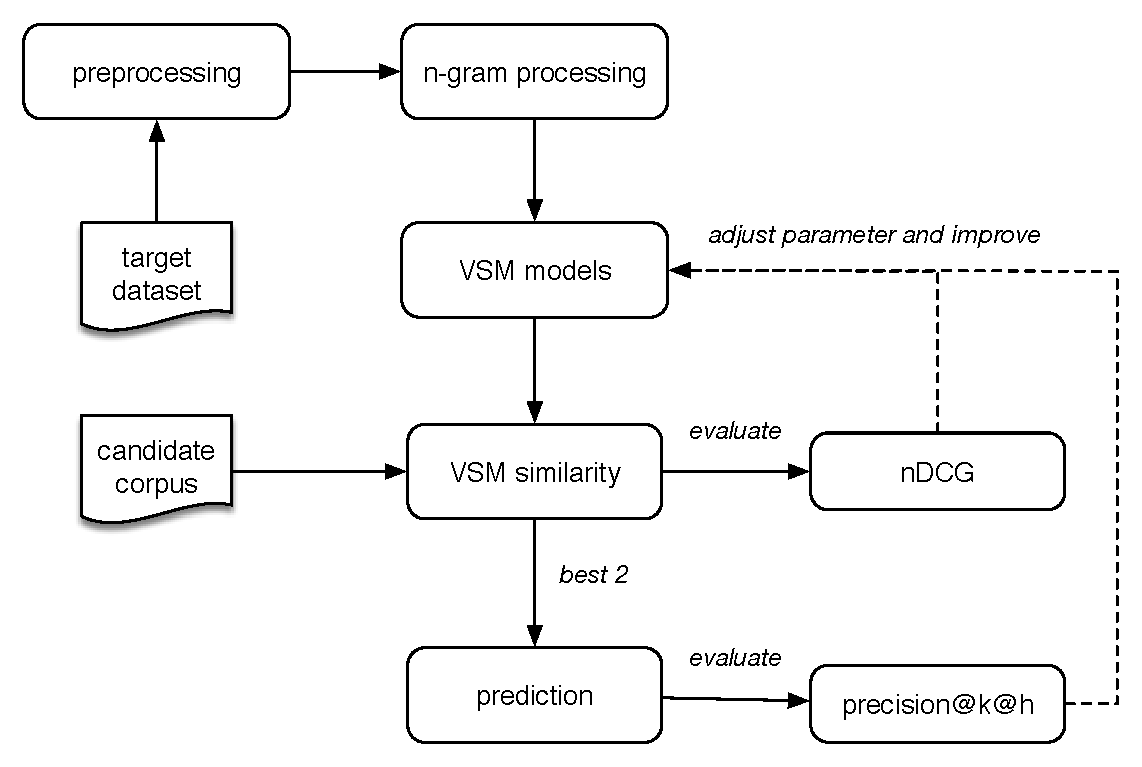
\includegraphics[width=0.7\textwidth]{fig/unsupervised}
    \caption{Caption}
    \label{fig:unsupervised}
\end{figure}



\subsection{Dataset}

The elementary structure and information is described in section \ref{sec:3.1}. Now we generate the dataset as the input of the framework. Articles, which have no related articles or no \textit{title}, or whose content is less than 1000 characters, are filtered. Furthermore, articles which belong to a weak category \footnote{Weak category: the amount of articles in this category is fewer than $1\%$ of the corpus size} or which were released before 2009 are removed from the corpus. We have $75908$ articles in $7$ categories. The category distribution is drawn in table \ref{tab:cate_dist_new} and the release date distribution is in table \ref{tab:release_dist_new}

\begin{table}[!htb]
\centering
\begin{tabular}{lrr}
\hline
\textbf{category} &   \textbf{quantity} &   \textbf{proportion (\%)} \\
\hline
Politik      &      26071 &            34.35 \\
Wirtschaft   &      12531 &            16.51 \\
Kultur       &       8584 &            11.31 \\
Gesellschaft &       7646 &            10.07 \\
Wissen       &       5273 &             6.95 \\
Sport        &       4993 &             6.58 \\
Digital      &       3887 &             5.12 \\
Reisen       &       2199 &             2.90 \\
Karriere     &       2169 &             2.86 \\
Studium      &       1570 &             2.07 \\
Lebensart    &        985 &             1.30 \\
\hline
\textbf{total}        &      75908 &           100.00 \\
\hline
\end{tabular}
\caption{Category distribution of \textit{ZEIT} corpus after filtering unsatisfied articles}
\label{tab:cate_dist_new}
\end{table}
\begin{table}[!htb]
\centering
\begin{tabular}{rrr}
\hline
\textbf{year} &   \textbf{quantity} &   \textbf{proportion (\%)} \\
\hline
2009 & 12628 &            16.64 \\
2010 & 14716 &            19.39 \\
2011 & 13970 &            18.40 \\
2012 & 14583 &            19.21 \\
2013 & 14941 &            19.68 \\
2014 &  5070 &             6.68 \\
\hline
\textbf{total} & 75908 &           100.00 \\
\hline
\end{tabular}
\caption{Release date distribution of \textit{ZEIT} corpus after filtering unsatisfied articles}
\label{tab:release_dist_new}
\end{table}

\begin{description}
\item[Experiment 1] $2000$ articles are selected randomly from the corpus as the test dataset, and the others are as the history data which is utilized to build unsupervised models. After that, the scores of relatedness of the tested articles are as the training dataset of supervised models. The supervised models will be trained by these data in the cross-validation way. 
\item[Experiment 2] The articles in corpus are sorted by the \textit{release date}, so that the real-world scenario can be simulated. The articles, which were published before 2013, are as the training data to initialize unsupervised models. There are two phases to deal with each target article, that are predicting related articles from the historical corpus and updating the model incrementally. Then the supervised methods make use of the scores from the unsupervised methods to compute the integrated scores and discover the related articles for each target article. 
\end{description}

\subsection{Preprocessing Methods}

The original content of articles is in the hypertext markup language format (HTML). The first common phase of preprocessing is to remove all markups and make the content case insensitive, in order to make the content in the simple text format. The second common phase, denoted as \textbf{\textit{split2word}}, is to split the content, also inclusive the title and the summary, into a sequence of tokens. The next two phases are optional and need evaluating. One is to filter out the stopwords, denoted as \textbf{\textit{stopword}}, which are most common words in a language, such as pronouns and prepositions. After removing the stopwords, the last phase \textbf{\textit{stem}} is to replace works by the stem thereof. For example, ``book'' is the stem of ``books'', ``booking'' and ``bookful'' and ``beauti'' is the stem of ``beauty'', ``beautiful'' and ``beautifully''. The advantage of stemming is to reduce the vocabulary size and furthermore decrease computational complexity and avoid overfitting of building semantic models. 

\subsection{Features}

\subsubsection{Meta-data}

\subsubsection{Semantic Features}

\subsection{Supervised Methods}


